\documentclass[11pt]{article}

\usepackage{abstract}
\usepackage{algorithm}
\usepackage{algorithmic}
\usepackage{amsmath}
\usepackage{amssymb}
\usepackage{bm}
\usepackage{caption}
\usepackage{CJKutf8}
\usepackage{color}
\usepackage{enumitem}
\usepackage{epsfig}
\usepackage{fancyhdr}
\usepackage{float}
\usepackage{graphics}
\usepackage{graphicx}
\usepackage{geometry}
\usepackage{indentfirst}
\usepackage{lastpage}
\usepackage{listings}
\usepackage{mathdots}
\usepackage{mathpazo}
\usepackage{multirow}
\usepackage{pstricks-add}
\usepackage{pst-blur}
\usepackage{subcaption}
\usepackage{tikz}
\usepackage{wasysym}
\usepackage{xcolor}
\usepackage[BoldFont,SlantFont,CJKsetspaces,CJKchecksingle]{xeCJK}

\allowdisplaybreaks
\DeclareMathOperator*{\argmin}{argmin}
\definecolor{Blue}{rgb}{1.,0.75,0.8}
\definecolor{mygray}{rgb}{0.5,0.5,0.5}
\definecolor{mygreen}{rgb}{0,0.6,0}
\definecolor{mymauve}{rgb}{0.58,0,0.82}
\pagestyle{empty}
\parindent 2em   %段首缩进
\setlength{\parindent}{2em}
\setCJKmainfont[BoldFont=SimHei]{SimSun}
\setCJKmonofont{SimSun}% 设置缺省中文字体
\usetikzlibrary{arrows, automata, calc, shapes}

\newcommand{\HRule}{\rule{\linewidth}{0.5mm}}
\newcommand{\hytt}[1]{\texttt{\hyphenchar\font=\defaulthyphenchar #1}}
\renewcommand{\algorithmicrequire}{\textbf{Input:}}   
\renewcommand{\algorithmicensure}{\textbf{Output:}}  
% \hyphenation{read-Sym-bol re-ad-Space-Tab-New-line str-Tab}

%\footnotesize
\lstset{ %
  backgroundcolor=\color{white},   % choose the background color; you must add \usepackage{color} or \usepackage{xcolor}
  basicstyle=\ttfamily,            % the size of the fonts that are used for the code
  breakatwhitespace=false,         % sets if automatic breaks should only happen at whitespace
  breaklines=true,                 % sets automatic line breaking
  captionpos=b,                    % sets the caption-position to bottom
  commentstyle=\ttfamily\color{mygreen},    
                                   % comment style
  deletekeywords={},               % if you want to delete keywords from the given language
  escapeinside={},                 % if you want to add LaTeX within your code
  extendedchars=true,              % lets you use non-ASCII characters; for 8-bits encodings only, does not work with UTF-8
  frame=single,                    % adds a frame around the code
  keepspaces=true,                 % keeps spaces in text, useful for keeping indentation of code (possibly needs columns=flexible)
  keywordstyle=\color{blue},       % keyword style
  language=C++,                    % the language of the code
  morekeywords={},                 % if you want to add more keywords to the set
  numbers=left,                    % where to put the line-numbers; possible values are (none, left, right)
  numbersep=5pt,                   % how far the line-numbers are from the code
  numberstyle=\tiny\color{mygray}, % the style that is used for the line-numbers
  rulecolor=\color{black},         % if not set, the frame-color may be changed on line-breaks within not-black text (e.g. comments (green here))
  showspaces=false,                % show spaces everywhere adding particular underscores; it overrides 'showstringspaces'
  showstringspaces=false,          % underline spaces within strings only
  showtabs=false,                  % show tabs within strings adding particular underscores
  stepnumber=1,                    % the step between two line-numbers. If it's 1, each line will be numbered
  stringstyle=\color{mymauve},     % string literal style
  tabsize=2,                       % sets default tabsize to 2 spaces
  title=\lstname                   % show the filename of files included with \lstinputlisting; also try caption instead of title
}

\pagestyle{fancy}
\rhead{page \thepage\ of \pageref{LastPage}}
%\chead{}
\lhead{操作系统实验报告}
\cfoot{}

\begin{document}

\title{操作系统实验5 \quad 页面置换算法}
\author{计算机1202 \quad 张艺瀚\\学号:20123852}
\maketitle

\thispagestyle{fancy}
%\newpage
\normalsize 

% 题目,目的,内容,要求 
% 程序流程图 
% 程序源代码、文档注释及文字说明 
% 运行结果及其说明 
% 回答以下问题: 
% 父进程空间与子进程空间的关系。 
% 通过完成实验,根据你的体会,阐述虚拟存储器的原理。 
% 写出FIFO算法中出现Belady现象的内存页面访问序列 

\section{实验题目}
编程实现FIFO和LRU算法

\section{实验目的}
\begin{enumerate}
\item 进一步理解父子进程之间的关系 
\item 理解内存页面调度的机理 
\item 掌握页面置换算法的实现方法 
\item 通过实验比较不同调度算法的优劣 
\item 培养综合运用所学知识的能力
\end{enumerate}

页面置换算法是虚拟存储管理实现的关键,通过本次试验理解内存页面调度的机制,在模拟实现FIFO、LRU等经典页面置换算法的基础上,比较各种置换算法的效率及优缺点,从而了解虚拟存储实现的过程。将不同的置换算法放在不同的子进程中加以模拟,培养综合运用所学知识的能力

\section{实验内容及要求}
\begin{enumerate}
  \item 这是一个综合型实验,要求在掌握父子进程并发执行机制和内存页面置换算法的基础上,能综合运用这两方面的知识,自行编制程序 
  \item 程序涉及一个父进程和两个子进程。父进程使用rand()函数随机产生若干随机数,经过处理后,存于一数组Acess\_Series[]中,作为内存页面访问的序列。两个子进程根据这个访问序列,分别采用FIFO和LRU两种不同的页面置换算法对内存页面进行调度。要求:
    \begin{enumerate}
      \item 
        \begin{enumerate}
          \item 设缺页的次数为diseffect。总的页面访问次数为total\_instruction。
          \item 缺页率 = disaffect/total\_instruction
          \item 命中率 = 1- disaffect/total\_instruction 
        \end{enumerate}
      \item 将为进程分配的内存页面数mframe作为程序的参数,通过多次运行程序,说明FIFO算法存在的Belady现象。
    \end{enumerate}
\end{enumerate}

\section{程序流程图}
见图\ref{fig: main}

\tikzstyle{startstop} = [rectangle, rounded corners, minimum width=2cm, minimum height=1cm,text centered, draw=black, fill=red!30]
\tikzstyle{io} = [trapezium, trapezium left angle=70, trapezium right angle=110, minimum width=2cm, minimum height=1cm, text centered, draw=black, fill=blue!30]
\tikzstyle{operation} = [rectangle, minimum width=2cm, minimum height=1cm, text centered, draw=black, fill=orange!30]
\tikzstyle{judge} = [diamond, minimum width=2cm, minimum height=1cm, text centered, draw=black, fill=green!30]
\tikzstyle{arrow} = [thick,->,>=stealth]

\begin{figure}[htbp]
\centering
\begin{tikzpicture}[node distance=2cm]
%定义流程图具体形状
\node (a) [startstop] at(0,1)      {开始};
\node (b) [operation] at(0,-0.5)      {随机生成访问序列};
\node (c) [operation] at(0,-2)      {创建子进程1};
\node (d) [judge] at(0,-5)      {\begin{tabular}{c} 子进程1 \\ 被调度? \end{tabular}};
\node (e) [operation] at(0,-7 - 1)      {\begin{tabular}{c} 按LRU调页 \\ (命中时调整 \\ 栈内顺序) \end{tabular}};
\node (f) [operation] at(0,-8.5 - 1.5)      {计算命中率};
\node (g) [operation] at(0,-10 - 1.5)      {子进程1结束};

\node (i) [operation] at(5,-2)      {创建子进程2};
\node (j) [judge] at(5,-5)      {\begin{tabular}{c} 子进程2 \\ 被调度? \end{tabular}};
\node (k) [operation] at(5,-7 - 1)      {\begin{tabular}{c} 按FIFO调页 \\ (命中时不调整 \\ 栈内顺序) \end{tabular}};
\node (l) [operation] at(5,-8.5 - 1.5)      {计算命中率};
\node (m) [operation] at(5,-10 - 1.5)      {子进程2结束};

\node (s) [startstop] at(5,-13)      {结束};

%连接具体形状
\draw [arrow](a) -- (b);
\draw [arrow](b) -- (c);
\draw [arrow](c) -- (d);
\draw [arrow](d) -- node[anchor=east] {Y} (0, -7) -- (e);
\draw [arrow](d) -- node[anchor=south] {N} (-3, -5) -- (-3, -12.5) -- (0, -12.5);
\draw [arrow](e) -- (f);
\draw [arrow](f) -- (g);

\draw [arrow](g) -- (0, -12.5) -- (2, -12.5) -- (2, -1) -- (5, -1) -- (i);

\draw [arrow](i) -- (j);
\draw [arrow](j) -- node[anchor=east] {Y} (5, -7) -- (k);
\draw [arrow](j) -- node[anchor=south] {N} (3, -5) -- (3, -12.25) -- (5, -12.25);
\draw [arrow](k) -- (l);
\draw [arrow](l) -- (m);
\draw [arrow](m) -- (s);

% \draw [arrow](n) -- (5, -13.5) -- (7.5, -13.5) -- (7.5, -7) -- (10, -7) -- (o);

% \draw [arrow](o) -- (p);
% \draw [arrow](p) -- (q);
% \draw [arrow](q) -- (r);
% \draw [arrow](r) -- (s);

%\draw [arrow]( ) -- node[anchor=east] {是} ( );
%\draw [arrow]( ) -- node[anchor=south] {否} ( );
\end{tikzpicture}
\caption{主过程}
\label{fig: main}
\end{figure}

\section{源程序}
\begin{lstlisting}[caption = {代码清单}, label = {lst: code}]
#include <stdio.h>
#include <sys/types.h>
#include <stdlib.h>
#include <sys/stat.h>
#include <fcntl.h>
#include <error.h>
#include <wait.h>
#include <unistd.h>

#include <algorithm>
#include <cassert>
#include <cmath>
#include <ctime>
#include <initializer_list>
#include <iostream>
#include <fstream>
#include <functional>
#include <set>
#include <sstream>
#include <vector>

using namespace std;

const int total_instruction = 10;
const int mem_frame_num = 4;
const int access_frame_num = 5;

template<typename T>
void disp(const vector<T>& vec){
  for_each(vec.begin(), vec.end(),
    [](const T& t){
      cout << t << " ";
    });
}

int main(int argc, char** argv){
  vector<int> access_series(total_instruction);
  srand(time(0));
  for(int i = 0; i < access_series.size(); ++i){
    access_series[i] = rand() % access_frame_num + 1;
  }
  cout << "access_series: ";
  disp(access_series);
  cout << endl;
  vector<int> fifo, lru;
  int p1, p2;
  while((p1 = fork()) == -1);
  if(p1 == 0){
    int disaffect = 0;
    double hit = 0;
    for(int i = 0; i < access_series.size(); ++i){
      cout << "lru\taccess frame " << access_series[i] << ";\t";
      auto pos = find(lru.begin(), lru.end(), access_series[i]);
      if(pos == lru.end()){
        if(lru.size() >= mem_frame_num){
          lru.erase(lru.begin());
        }
        lru.push_back(access_series[i]);
        ++disaffect;
        cout << "disaffect = " << disaffect << "\t";
        disp(lru); cout << endl;
      }else{
        lru.erase(pos);
        lru.push_back(access_series[i]);
        cout << "\t\t";
        disp(lru);
        cout << endl;
      }
    }
    hit = 1 - disaffect * 1.0 / total_instruction;
    cout << "lru\thit = " << hit << endl;
    exit(0);
  }
  while((p2 = fork()) == -1);
  if(p2 == 0){
    int disaffect = 0;
    double hit = 0;
    for(int i = 0; i < access_series.size(); ++i){
      cout << "fifo\taccess frame " << access_series[i] << ";\t";
      auto pos = find(fifo.begin(), fifo.end(), access_series[i]);
      if(pos == fifo.end()){
        if(fifo.size() >= mem_frame_num){
          fifo.erase(fifo.begin());
        }
        fifo.push_back(access_series[i]);
        ++disaffect;
        cout << "disaffect = " << disaffect << "\t";
        disp(fifo); cout << endl;
      }else{
        cout << "\t\t";
        disp(fifo);
        cout << endl;
      }
    }
    hit = 1 - disaffect * 1.0 / total_instruction;
    cout << "fifo\thit = " << hit << endl;
    exit(0);
  }
  return 0;
}
\end{lstlisting}

\section{运行结果及其说明}
\begin{tabular}{ c|cccc|c|cccc|c }
\hline
访问页 & \multicolumn{4}{ |c| }{LRU} & 命中 & \multicolumn{4}{ |c| }{FIFO} & 命中 \\ \hline
5 & 5 &   &   &   & $\times    $ & 5 &   &   &   & $\times    $ \\ \hline
1 & 5 & 1 &   &   & $\times    $ & 5 & 1 &   &   & $\times    $ \\ \hline
5 & 1 & 5 &   &   & $\checkmark$ & 5 & 1 &   &   & $\checkmark$ \\ \hline
2 & 1 & 5 & 2 &   & $\times    $ & 5 & 1 & 2 &   & $\checkmark$ \\ \hline
1 & 5 & 2 & 1 &   & $\checkmark$ & 5 & 1 & 2 &   & $\checkmark$ \\ \hline
5 & 2 & 1 & 5 &   & $\checkmark$ & 5 & 1 & 2 &   & $\checkmark$ \\ \hline
1 & 2 & 5 & 1 &   & $\checkmark$ & 5 & 1 & 2 &   & $\checkmark$ \\ \hline
4 & 2 & 5 & 1 & 4 & $\times    $ & 5 & 1 & 2 & 4 & $\times    $ \\ \hline
1 & 2 & 5 & 4 & 1 & $\checkmark$ & 5 & 1 & 2 & 4 & $\checkmark$ \\ \hline
4 & 2 & 5 & 1 & 4 & $\checkmark$ & 5 & 1 & 2 & 4 & $\checkmark$ \\ \hline
\end{tabular}

\begin{center}
\begin{figure}[htbp]
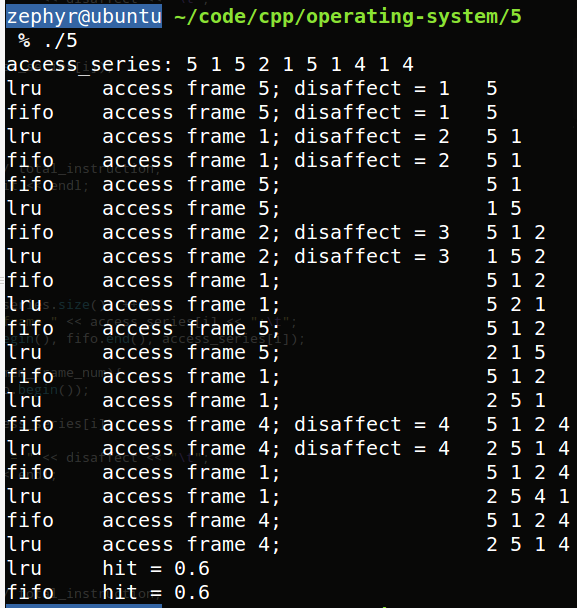
\includegraphics[width=\textwidth]{lru_fifo.png}
\caption{运行结果}
\label{fig: pipe}
\end{figure}
\end{center}

\section{回答问题}
\subsection{父进程空间与子进程空间的关系。}
使用fork创建子进程时,逻辑上,除了pid和父进程的一些不允许共享的数据外,子进程的pcb几乎是父进程pcb的精确复制,它们具有相同的代码、数据、现场、资源等等;物理上,并不会为子进程另外开辟一段内存空间将父进程复制一份,而是二者通过一定的控制共享同一个进程空间。父子进程和系统中的其他进程并发执行,调度顺序由操作系统调度程序决定,不受用户干预,可以通过fork的返回值区分它们,子进程从fork语句的下一条开始指令行开始执行。

\subsection{通过完成实验,根据你的体会,阐述虚拟存储器的原理。}
\begin{enumerate}
  \item 部分调入:程序装入时,不必一次性全部装入内存,而是允许部分装入就开始执行;
  \item 现用现调:程序执行过程中如果访问的指令(数据)不在内存,产生缺页(段)中断,将需要的页(段)调入内存;
  \item 不够换出:内存紧张时,将一些页(段)换出内存,从而装入需要调入的页(段)。
\end{enumerate}

\subsection{写出FIFO算法中出现Belady现象的内存页面访问序列。}
\begin{tabular}{ c|ccc|c|cccc|c }
\hline
访问页 & \multicolumn{3}{ |c| }{FIFO1} & 命中 & \multicolumn{4}{ |c| }{FIFO2} & 命中 \\ \hline
1 & 1 &   &   & $\times    $ & 1 &   &   &   & $\times    $ \\ \hline
2 & 2 & 1 &   & $\times    $ & 2 & 1 &   &   & $\times    $ \\ \hline
3 & 3 & 2 & 1 & $\times    $ & 3 & 2 & 1 &   & $\times    $ \\ \hline
4 & 4 & 3 & 2 & $\times    $ & 4 & 3 & 2 & 1 & $\times    $ \\ \hline
1 & 1 & 4 & 3 & $\times    $ & 4 & 3 & 2 & 1 & $\checkmark$ \\ \hline
2 & 2 & 1 & 4 & $\times    $ & 4 & 3 & 2 & 1 & $\checkmark$ \\ \hline
5 & 5 & 2 & 1 & $\times    $ & 5 & 4 & 3 & 2 & $\times    $ \\ \hline
1 & 5 & 2 & 1 & $\checkmark$ & 1 & 5 & 4 & 3 & $\times    $ \\ \hline
2 & 5 & 2 & 1 & $\checkmark$ & 2 & 1 & 5 & 4 & $\times    $ \\ \hline
3 & 3 & 5 & 2 & $\times    $ & 3 & 2 & 1 & 5 & $\times    $ \\ \hline
4 & 4 & 3 & 5 & $\times    $ & 4 & 3 & 2 & 1 & $\times    $ \\ \hline
5 & 4 & 3 & 5 & $\checkmark$ & 5 & 4 & 3 & 2 & $\times    $ \\ \hline
\end{tabular}

\end{document}
